\subsubsection{Liberación secuencial}

\lipsum[1]

    \begin{figure}[!h]
        \centering
        
\includegraphics[width=1\textwidth]{Figuras/secuencial_1}
        \centering\caption{Liberación secuencial.}
        \label{fig:secuencial_1}
    \end{figure}
    
\lipsum[1]

    \begin{figure}[!h]
        \centering
        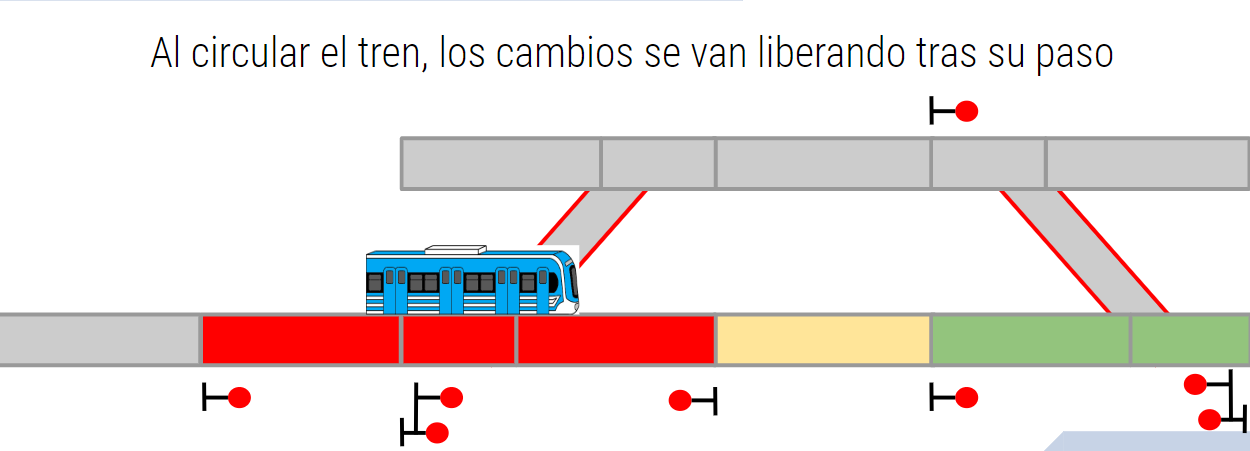
\includegraphics[width=1\textwidth]{Figuras/secuencial_2}
        \centering\caption{Liberación secuencial.}
        \label{fig:secuencial_2}
    \end{figure}
    
\lipsum[1]

    \begin{figure}[!h]
        \centering
        
\includegraphics[width=1\textwidth]{Figuras/secuencial_3}
        \centering\caption{Liberación secuencial.}
        \label{fig:secuencial_3}
    \end{figure}
    
\lipsum[1]

    \begin{figure}[!h]
        \centering
        
\includegraphics[width=1\textwidth]{Figuras/secuencial_4}
        \centering\caption{Liberación secuencial.}
        \label{fig:secuencial_4}
    \end{figure}
    
\lipsum[1]